\documentclass{article}
\usepackage[utf8]{inputenc}
\usepackage{amsmath}
\usepackage{amssymb}
\usepackage{geometry}
\usepackage{graphicx}
\usepackage{float}
\usepackage{tikz}
\usetikzlibrary{shapes.geometric, arrows, positioning, calc, patterns}

\geometry{a4paper, margin=1in}

\title{Model Extension: Author-Journal Game with Competition and Capacity Constraints}

\date{\today}

\begin{document}

\maketitle

\section{Motivation and Problem Statement}

In our previous evolutionary game-theoretic model of the author-journal interaction, we observed that the equilibrium strategies were largely insensitive to the population size $N$. This phenomenon arises because, in the original formulation, the payoff of a focal author depends solely on their own strategy and the journal's acceptance policy, but is independent of the actions of other authors. Consequently, there is no \textit{congestion effect} or \textit{competition} for limited resources.

To address this and model a more realistic academic publishing environment (e.g., conferences with fixed acceptance rates or journals with limited pages), we introduce a capacity threshold $K$. This mechanism creates a zero-sum element: as the number of submissions increases, the probability of acceptance for a passed paper decreases, potentially disincentivizing opportunistic strategies like \textit{Always Submit} (AS).

\section{The Threshold Competition Model}


The updated interaction proceeds in the following stages:
\begin{enumerate}
    \item \textbf{Submission:} $N$ authors choose a strategy $s \in \{OG, AS, \dots\}$.
    \item \textbf{Peer Review (Perception):} All submissions undergo peer review characterized by false negative rate $\epsilon$ and false positive rate $\lambda$. Papers that pass peer review enter a ``Perception Pool'' of size $M$.
    \item \textbf{Competition (Threshold Cut):} The journal has a maximum capacity $K$.
    \begin{itemize}
        \item If $M \le K$, all papers in the pool are accepted.
        \item If $M > K$, the journal randomly selects $K$ papers from the pool to accept. The remaining $M-K$ papers are rejected despite passing review.
    \end{itemize}
\end{enumerate}


Let $\alpha$ be the probability an author produces a good paper. The probability that a single author's submission passes the peer review stage, denoted as $P_{pass}(s)$, depends on their chosen strategy $s$:

\begin{align}
    P_{pass}(OG) &= \alpha(1-\epsilon) \\
    P_{pass}(AS) &= \alpha(1-\epsilon) + (1-\alpha)\lambda
\end{align}

Here, $OG$ authors only submit good papers, while $AS$ authors submit both good and bad papers, benefiting from the false positive rate $\lambda$.


\begin{figure}[htbp]
    \centering
    % 这一行让图片自动缩放适应页面宽度
    \resizebox{\textwidth}{!}{
        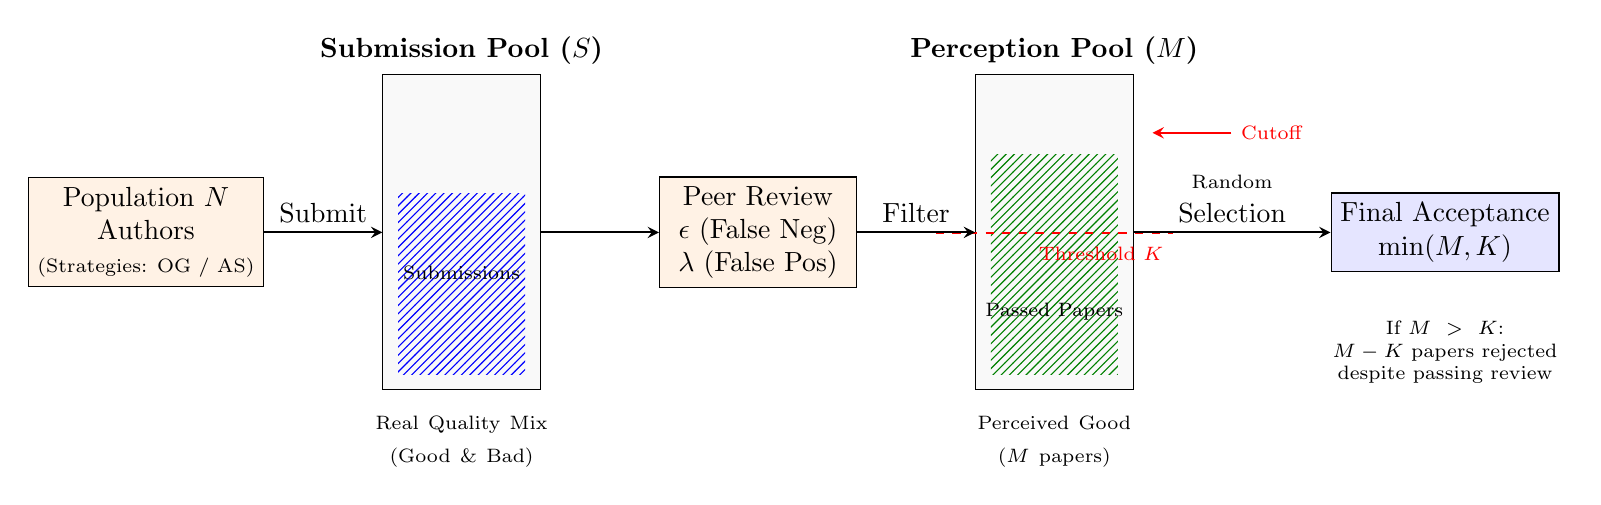
\begin{tikzpicture}[node distance=2cm, auto, >=stealth]

        % --- 定义样式 ---
        \tikzstyle{process} = [rectangle, minimum width=2.5cm, minimum height=1cm, text centered, draw=black, fill=orange!10]
        \tikzstyle{pool} = [rectangle, minimum width=2cm, minimum height=4cm, draw=black, fill=gray!5]
        \tikzstyle{arrow} = [thick,->]

        % --- 节点定义 ---

        % 1. Authors
        \node (authors) [process, align=center] {Population $N$ \\ Authors \\ \scriptsize (Strategies: OG / AS)};

        % 2. Submission Pool
        \node (submit_pool) [pool, right=1.5cm of authors, label=above:\textbf{Submission Pool ($S$)}] {};
        \fill[pattern=north east lines, pattern color=blue] ($(submit_pool.south west) + (0.2,0.2)$) rectangle ($(submit_pool.south east) + (-0.2, 2.5)$);
        \node at ($(submit_pool.south) + (0, 1.5)$) {\scriptsize Submissions};

        % 3. Peer Review
        \node (review) [process, right=1.5cm of submit_pool, align=center] {Peer Review \\ $\epsilon$ (False Neg) \\ $\lambda$ (False Pos)};

        % 4. Perception Pool
        \node (percep_pool) [pool, right=1.5cm of review, label=above:\textbf{Perception Pool ($M$)}] {};
        \fill[pattern=north east lines, pattern color=green!50!black] ($(percep_pool.south west) + (0.2,0.2)$) rectangle ($(percep_pool.south east) + (-0.2, 3.0)$);
        \node at ($(percep_pool.south) + (0, 1.0)$) {\scriptsize Passed Papers};

        % --- Threshold K (红色虚线与文字) ---
        \draw[red, thick, dashed] ($(percep_pool.south west) + (-0.5, 2.0)$) -- ($(percep_pool.south east) + (0.5, 2.0)$);
        % 文字在虚线右下方
        \node[text=red, anchor=north east, yshift=-0.05cm] at ($(percep_pool.south east) + (0.5, 2.0)$) {\scriptsize Threshold $K$};

        % 5. Final Selection
        \node (final) [process, right=2.5cm of percep_pool, align=center, fill=blue!10] {Final Acceptance \\ $\min(M, K)$};

        % --- 连线 ---
        \draw[arrow] (authors) -- node[above] {Submit} (submit_pool);
        \draw[arrow] (submit_pool) -- (review);
        \draw[arrow] (review) -- node[above] {Filter} (percep_pool);

        % --- Cutoff (Cutoff 在 Random Selection 上方,箭头向左) ---
        \draw[arrow] (percep_pool) -- node[above, align=center] (rand_sel) {\scriptsize Random\\Selection} (final);
        
        % Label
        \node[above=0.2cm of rand_sel, xshift=0.5cm, text=red] (cutoff_label) {\scriptsize Cutoff};
        % Arrow pointing LEFT
        \draw[->, red, thick] (cutoff_label.west) -- ++(-1.0, 0);

        % --- 底部注释 ---
        \node [below=0.2cm of submit_pool, text width=2.5cm, align=center] {\scriptsize Real Quality Mix\\(Good \& Bad)};
        \node [below=0.2cm of percep_pool, text width=2.5cm, align=center] {\scriptsize Perceived Good\\($M$ papers)};
        \node [below=0.5cm of final, text width=3cm, align=center, font=\scriptsize] {If $M > K$: \\ $M-K$ papers rejected \\ despite passing review};

        \end{tikzpicture}
    }
    \caption{\textbf{Schematic representation of the Threshold Competition Model.} The process unfolds in three stages: (1) Submission into a pool $S$; (2) Peer review filtering into a perception pool $M$; and (3) A hard capacity constraint $K$ (red dashed line). If $M > K$, a random cutoff occurs, rejecting surplus papers even if they passed review. This introduces the competition factor $\gamma$.}
    \label{fig:threshold_model}
\end{figure}
\section{Derivation of the Competition Factor $\gamma$}

The key addition to the payoff function is the competition factor $\gamma$, which represents the probability that a paper is finally accepted \textit{given that it has already passed peer review}.

Let us consider a \textit{focal author} who has passed peer review. Let $M_{-i}$ be the random variable representing the number of \textit{other} authors (out of $N-1$) whose papers also passed peer review.

The total number of passed papers is therefore $M = 1 + M_{-i}$.

The competition factor for the focal author is defined as:
\begin{equation}
    \gamma_{\text{focal}} = \min\left(1, \frac{K}{1 + M_{-i}}\right) = 
    \begin{cases} 
      1 & \text{if } 1 + M_{-i} \le K \\
      \frac{K}{1 + M_{-i}} & \text{if } 1 + M_{-i} > K
   \end{cases}
\end{equation}

\subsection{Expected Competition Factor}
Since $M_{-i}$ is a random variable, authors base their decisions on the expected value $E[\gamma_{\text{focal}}]$. 

Assume the population consists of $N_{OG}$ authors playing $OG$ and $N_{AS}$ authors playing $AS$ (where $N_{OG} + N_{AS} = N - 1$, excluding the focal author). The variable $M_{-i}$ is the sum of two independent binomial distributions:
\begin{equation}
    M_{-i} = X_{OG} + X_{AS}
\end{equation}
where $X_{OG} \sim B(N_{OG}, P_{pass}(OG))$ and $X_{AS} \sim B(N_{AS}, P_{pass}(AS))$.

The expected competition factor is given by:
\begin{equation}
    E[\gamma_{\text{focal}}] = \sum_{m=0}^{N-1} \Pr(M_{-i} = m) \cdot \min\left(1, \frac{K}{1 + m}\right)
\end{equation}



\section{Derivation of Dominated Strategies}

In this section, we provide a detailed mathematical derivation to justify the reduction of the strategy space. We demonstrate that under specific parameter constraints, the strategies \textit{Only Bad} (OB), \textit{Never Submit} (NS), and \textit{Always Accept} (AA) are strictly dominated.



We define the following parameters governing the author-journal game:
\begin{itemize}
    \item $\alpha$: The probability that an author produces a high-quality paper.
    \item $\gamma$: The competition factor, representing the probability of acceptance after passing peer review ($0 < \gamma \le 1$).
    \item $r$: The reward for an author when a paper is accepted.
    \item $c$: The cost of submission incurred by the author.
    \item $\epsilon$: The false negative rate (probability that a good paper is rejected).
    \item $\lambda$: The false positive rate (probability that a bad paper is accepted).
    \item $B$: The benefit to the journal for accepting a good paper.
    \item $D$: The penalty to the journal for accepting a bad paper.
\end{itemize}



The set of possible strategies for an author is $S_A \in \{OG, AS, OB, NS\}$.



We compare the expected utility of the \textit{Only Bad} (OB) strategy against the \textit{Never Submit} (NS) strategy.
\begin{itemize}
    \item \textbf{Payoff for NS:} $U_A(NS) = 0$.
    \item \textbf{Payoff for OB:} An author using OB only submits bad papers (probability $1-\alpha$). A bad paper is accepted only if it passes peer review (probability $\lambda$) and survives the competition threshold (probability $\gamma$).
\end{itemize}

The expected utility is:
\begin{equation}
    U_A(OB) = (1-\alpha) \cdot [ (\lambda \cdot \gamma \cdot r) - c ]
\end{equation}

For $NS$ to strictly dominate $OB$, we require $U_A(NS) > U_A(OB)$ for any state of the system.
\begin{align}
    0 &> (1-\alpha) \cdot [ \lambda \gamma r - c ] \\
    \text{Since } (1-\alpha) > 0, \quad 0 &> \lambda \gamma r - c \notag \\
    c &> \lambda \gamma r \label{eq:ob_derive}
\end{align}

Since $\gamma$ is a variable representing congestion ($\gamma \in (0, 1]$), we must ensure this inequality holds even in the "best-case scenario" for a bad paper, which occurs when there is no competition ($\gamma = 1$). Substituting $\max(\gamma) = 1$ into Inequality (\ref{eq:ob_derive}), we derive the sufficient condition:

\begin{equation}
    \boxed{c > \lambda \cdot r}
\end{equation}

\textbf{Conclusion:} If the submission cost $c$ is strictly greater than the maximum theoretical reward of a bad paper passing review ($\lambda r$), $U_A(OB)$ is always negative. Thus, $OB$ is strictly dominated by $NS$.


We compare \textit{Only Good} (OG) against \textit{Never Submit} (NS).
\begin{itemize}
    \item \textbf{Payoff for OG:} An author submits only good papers (probability $\alpha$). It is accepted if it passes review (probability $1-\epsilon$) and survives competition ($\gamma$).
\end{itemize}

The expected utility is:
\begin{equation}
    U_A(OG) = \alpha \cdot [ (1-\epsilon) \cdot \gamma \cdot r - c ]
\end{equation}

For $OG$ to strictly dominate $NS$, we require $U_A(OG) > U_A(NS) = 0$.
\begin{align}
    \alpha \cdot [ (1-\epsilon) \gamma r - c ] &> 0 \\
    (1-\epsilon) \gamma r - c &> 0 \notag \\
    (1-\epsilon) \gamma r &> c \notag \\
    \gamma &> \frac{c}{r(1-\epsilon)}
\end{align}

\textbf{Conclusion:} The dominance of $OG$ over $NS$ is conditional. We define the \textbf{Viability Condition}:
\begin{equation}
    \boxed{\gamma > \frac{c}{r(1-\epsilon)}}
\end{equation}
As long as the system congestion does not drive $\gamma$ below this critical threshold, the expected return of a high-quality paper covers the submission cost, making $OG$ the rational choice over $NS$.



We analyze the \textit{Always Accept} (AA) strategy. Under this strategy, the journal abandons screening ($\lambda=1, \epsilon=0$). Assuming authors may submit bad papers (e.g., under strategy AS), the pool of accepted papers reflects the natural distribution of paper quality ($\alpha$).

The journal's expected utility function $U_J$ (ignoring processing costs for simplicity) is:
\begin{equation}
    U_J(AA) = \text{Volume} \cdot [ \alpha \cdot B - (1-\alpha) \cdot D ]
\end{equation}

For $AA$ to be a dominated strategy (specifically, yielding negative utility compared to a selective strategy), we require $U_J(AA) < 0$:
\begin{align}
    \alpha \cdot B - (1-\alpha) \cdot D &< 0 \\
    \alpha \cdot B &< (1-\alpha) \cdot D \notag \\
    \frac{\alpha B}{1-\alpha} &< D \notag
\end{align}

Rearranging this gives the \textbf{Reputation Constraint}:
\begin{equation}
    \boxed{D > \frac{\alpha}{1-\alpha} B}
\end{equation}

\textbf{Conclusion:} If the penalty for accepting a bad paper ($D$) exceeds the benefit of a good paper ($B$) weighted by the odds of good-to-bad submissions ($\frac{\alpha}{1-\alpha}$), the $AA$ strategy yields negative utility. In such a regime, a journal must adopt a selective strategy ($OG\_J$) to remain viable.



In conclusion, the simplified game dynamics between $OG$ and $AS$ for authors, and the strict selection strategy for journals, are valid under the following parameter constraints:
\begin{enumerate}
    \item $c > \lambda r$ (Prevents malicious submission of bad papers).
    \item $\gamma > \frac{c}{r(1-\epsilon)}$ (Ensures good papers are profitable despite competition).
    \item $D > \frac{\alpha}{1-\alpha} B$ (Ensures journals are motivated to filter quality).
\end{enumerate}


The assumption that these constraints hold is strictly necessary to model a functional and sustainable scientific community rather than a degenerate system. Specifically, the condition $c > \lambda r$ ensures that the ecosystem is not overwhelmed by costless speculative spamming; the lower bound on $\gamma$ posits that the journal has not reached a state of total collapse where even high-quality contributions are discouraged; and the reputation constraint on $D$ distinguishes legitimate, quality-seeking venues from predatory publishers. By restricting our analysis to this valid parameter space, we filter out trivial breakdown scenarios to focus exclusively on the non-trivial evolutionary dynamics: how resource scarcity ($K$) and congestion precipitate a tragedy of the commons, and how the interplay between institutional screening and authorial strategy can resolve it.
\section{Updated Payoff Functions}

We incorporate $E[\gamma_{\text{focal}}]$ into the utility functions. Let $r$ be the reward for acceptance and $c$ be the cost of submission.


An $OG$ author submits with probability $\alpha$. If they submit, they pay cost $c$. They pass review with probability $1-\epsilon$. If they pass, they are accepted with probability $E[\gamma_{\text{focal}}]$.

\begin{equation}
    U_A(OG) = \alpha \left[ (1-\epsilon) \cdot E[\gamma_{\text{focal}}] \cdot r - c \right]
\end{equation}
\textit{Note: Assuming cost is paid per submission regardless of acceptance.}


An $AS$ author always submits (probability 1), paying cost $c$. They pass review with probability $P_{pass}(AS)$. If they pass, they are accepted with probability $E[\gamma_{\text{focal}}]$.

\begin{equation}
    U_A(AS) = \left[ (\alpha(1-\epsilon) + (1-\alpha)\lambda) \cdot E[\gamma_{\text{focal}}] \cdot r \right] - c
\end{equation}


The journal's utility depends on the quality of the final accepted papers and the cost of reviewing the total volume of submissions. 

Let $B$ be the benefit for accepting a good paper and $D$ be the penalty for accepting a bad paper.
The total submission volume $S$ is given by:
\begin{equation}
    E[S] = N_{OG} \cdot \alpha + N_{AS} \cdot 1
\end{equation}

The ``Perception Pool'' $M$ contains a mix of good and bad papers that passed review.
The expected number of good papers ($M_G$) and bad papers ($M_B$) in the pool are:
\begin{align}
    E[M_G] &= (N_{OG} + N_{AS}) \cdot \alpha(1-\epsilon) \\
    E[M_B] &= N_{AS} \cdot (1-\alpha)\lambda
\end{align}
\textit{Note: Both OG and AS authors contribute to $M_G$, but only AS authors contribute to $M_B$.}

Since the journal selects $K$ papers randomly from $M$ (if $M > K$), the final accepted papers maintain the same quality ratio as the pool. The expected acceptance rate for any paper in the pool is approximated by the system-wide competition factor $\bar{\gamma} = E[\min(1, K/M)]$.

The journal's expected payoff is:
\begin{equation}
    U_J = B \cdot (E[M_G] \cdot \bar{\gamma}) - D \cdot (E[M_B] \cdot \bar{\gamma}) - C(E[S])
\end{equation}

Where $C(S)$ is the cost function (e.g., linear or convex with respect to total submissions). This formulation highlights that while $K$ limits the absolute number of bad papers accepted (by reducing $\bar{\gamma}$), it does not improve the \textit{ratio} of good to bad papers, which is still determined by $\epsilon$ and $\lambda$.
\section{Discussion: The Effect of $N$}

In this new model, the population size $N$ plays a decisive role in shaping equilibrium outcomes, particularly when the journal's capacity $K$ remains fixed or grows at a slower rate than $N$. As the number of authors increases, the expected number of papers passing peer review, $E[M]$, naturally rises. This effect is exacerbated if authors adopt the \textit{Always Submit} (AS) strategy, which floods the perception pool with bad papers that pass due to the false positive rate $\lambda$. This surge in submissions shifts the probability distribution of $M_{-i}$ toward higher values, thereby mechanically reducing the expected competition factor $E[\gamma_{\text{focal}}]$. Consequently, the effective reward for publication is diluted. If $E[\gamma_{\text{focal}}]$ drops below a critical threshold, the expected benefit of the indiscriminate $AS$ strategy may no longer cover the submission cost $c$. This mechanism creates a congestion effect that can potentially restore the stability of the cooperative \textit{Only Good} (OG) strategy or, in extreme cases of overcrowding, lead to a \textit{No Submit} (NS) equilibrium. Thus, the model effectively reintroduces the ``tragedy of the commons,'' demonstrating that population size and finite resource constraints are fundamental determinants of stability in the academic publishing ecosystem.

\section{Determination of Capacity $K$}

The parameter $K$ represents the scarcity of resources (e.g., journal pages or conference presentation slots). To ensure the model reflects realistic dynamics, we propose determining $K$ through two complementary approaches: empirical anchoring and regime analysis.


We can calibrate $K$ based on historical data from top-tier venues. For instance, top computer science conferences (such as ICLR) typically maintain an acceptance rate between 20\% and 30\%. Therefore, in our simulations, we can anchor $K$ such that:
\begin{equation}
    K \approx \delta \cdot N, \quad \text{where } \delta \in [0.2, 0.3]
\end{equation}
This ensures the baseline competition level matches real-world observations.


To fully explore the strategic implications of competition, we analyze the model across three distinct capacity regimes:

\begin{itemize}
    \item \textbf{Resource Scarcity ($K \ll \alpha N$):} In this regime (e.g., $K \approx 0.1N$), competition is intense. The value of $\gamma$ is significantly less than 1 even if all authors cooperate (play OG). Here, the primary driver is the raw capacity constraint, which may force authors into $NS$ strategies to avoid sunk costs.
    
    \item \textbf{Balanced Resources ($K \approx \alpha N$):} This is the most strategically critical regime. The capacity is sufficient to accommodate most good papers, provided authors do not flood the system with bad ones. However, if a significant fraction of authors switches to $AS$, the system quickly becomes congested, causing $\gamma$ to drop. This regime highlights the tension between individual opportunism and collective efficiency.
    
    \item \textbf{Resource Abundance ($K \to N$):} When capacity is abundant (e.g., $K \ge 0.8N$), the competition factor $\gamma \to 1$. In this limit, the model converges back to our original formulation without the threshold constraint, serving as a control group to isolate the effects of competition.
\end{itemize}

\section{Simulation Analysis and Discussion}

Based on the theoretical framework of the Threshold Competition Model, we conducted numerical simulations to examine how the capacity constraint ($K$) and population size ($N$) shape strategic outcomes for authors and journals. This section summarises the simulation design and discusses the main qualitative patterns that emerge.

The simulation environment is constructed as a ``funnel selection'' process, mirroring the constraints of top-tier conferences. Unless stated otherwise, we use $N=100$, $K=20$, $\epsilon=\lambda=0.1$, $B=1.0$, and $D=3.0$. These values implement the following design choices:
\begin{itemize}
    \item \textbf{Funnel mechanism:} The process has three stages: a \emph{Submission Pool} ($S$) generated by $N$ authors; a \emph{Perception Pool} ($M$) filtered by noisy peer review; and a final \emph{Threshold Cut} in which at most $K$ papers are accepted.
    \item \textbf{Resource scarcity:} With $N=100$ and $K=20$, the baseline acceptance rate is only 20\%, creating intense competition for limited slots.
    \item \textbf{Peer-review noise:} Reviewers misclassify good and bad papers with probability $0.1$, providing a niche for the \textit{Always Submit} (AS) strategy to exploit false positives.
    \item \textbf{High penalty for bad papers:} The journal incurs a much larger loss for publishing a bad paper than it gains from a good one ($D>B$), capturing the incentives of reputation-sensitive venues.
\end{itemize}

To maintain mathematical control, we avoid Monte Carlo sampling and instead use two deterministic components:
\begin{enumerate}
    \item \textbf{Exact probability convolution.} For a given mixture of cooperative (OG) and opportunistic (AS) authors, the distribution of the number of passing papers $M_{-i}$ contributed by the rest of the population is obtained as the convolution of two binomial distributions. This yields an exact value for the expected competition factor $E[\gamma]$.
    \item \textbf{Coupled replicator dynamics.} Author strategies evolve according to the expected payoffs determined by $E[\gamma]$, while journal strategies simultaneously adapt their selectivity ($\phi_{OG}$) based on the expected quality of the accepted pool.
\end{enumerate}

\subsection{Static Analysis: Congestion and the Commons}

Figure~\ref{fig:static_analysis} presents the static analysis of the competition factor $E[\gamma]$, isolating the effects of strategy mix and population size.

\begin{figure}[htbp]
    \centering
    % 请确保使用静态分析图的文件名
    \includegraphics[width=\textwidth]{static_analysis.png}
    \caption{\textbf{Static analysis of competition.} \textbf{Left:} Decline of $E[\gamma]$ as the proportion of AS authors increases ($N=100$, $K=20$), illustrating a tragedy-of-the-commons effect. \textbf{Right:} Dependence of $E[\gamma]$ on population size $N$ (with $K=20$), highlighting the onset of congestion.}
    \label{fig:static_analysis}
\end{figure}

The right panel resolves the earlier anomaly that payoffs appeared insensitive to $N$ in simpler models. For small populations ($N\lesssim 40$), the expected number of passing papers remains below the capacity $K$, so $E[\gamma]=1$ and the capacity constraint is non-binding. In this pre-congestion regime, enlarging the population does not affect individual acceptance probabilities, which explains why purely linear models fail to detect any $N$-dependence. Once $N$ crosses the approximate saturation threshold $N \approx K / P_{pass}$, the system enters a congestion regime in which $E[\gamma]$ falls sharply towards $K/M \approx 0.2$. The threshold $K$ thus acts as a critical link between macroscopic population size and microscopic strategic payoffs.

The left panel shows how opportunism feeds back on itself. As the share of AS authors increases, both genuine contributions and false positives inflate the perception pool $M$. Because only $K$ papers can be accepted, the per-paper competition factor $\gamma = K/M$ shrinks for everyone. Individually profitable deviations towards AS therefore generate a tragedy-of-the-commons outcome at the population level.

\subsection{Co-evolutionary Dynamics}

Figure~\ref{fig:dynamic_evolution} turns to the full co-evolutionary dynamics of authors and journals.

\begin{figure}[htbp]
    \centering

    \includegraphics[width=\textwidth]{dynamic_evolution.png}
    \caption{\textbf{Co-evolutionary dynamics.} \textbf{Left:} Time series of the share of AS authors ($\theta_{AS}$, blue) and OG journals ($\phi_{OG}$, red dashed). \textbf{Right:} Phase-plane trajectory showing the specific evolution from the initial state $(\theta_{AS}=0.5, \phi_{OG}=0.5)$.}
    \label{fig:dynamic_evolution}
\end{figure}

The time series (left panel) reveals a clear separation of time scales. The journal population reacts almost instantly: under high penalties for bad publications and strong congestion ($K=20$), the \textit{Always Accept} policy becomes prohibitively costly, and journals rapidly converge to strict selection ($\phi_{OG}\approx 1$). By contrast, authors adapt more slowly. Starting from $\theta_{AS}=0.5$, the share of opportunistic authors gradually declines towards $\theta_{AS}\approx 0.2$ as AS becomes doubly penalised: first by strict peer review (via $\epsilon$), and second by the reduced competition factor ($\gamma<1$) caused by congestion.

\subsection{Global Stability and Robustness}

To ensure the observed outcome is robust to initial conditions, Figure~\ref{fig:phase_plane_global} provides a global view of the system's dynamics using a detailed phase plane.

\begin{figure}[!h]
    \centering
    \includegraphics[width=0.85\textwidth]{phase_plane_global.png}
    \caption{\textbf{Global stability analysis.} Phase-plane trajectories in the $(\theta_{AS},\phi_{OG})$ plane starting from various initial conditions (coloured lines). Grey streamlines represent the evolutionary vector field, indicating the direction of drift under replicator dynamics.}
    \label{fig:phase_plane_global}
\end{figure}

The horizontal axis represents the authors' behaviour (from fully cooperative on the left to fully opportunistic on the right); the vertical axis represents journal policy (from permissive at the bottom to strict at the top). Grey streamlines act as ``evolutionary currents,'' indicating the system's inherent drive at any given state.

Across all starting points, trajectories display a characteristic inverted ``L'' shape. They first move almost vertically upward as journals swiftly adopt strict screening, and only then drift horizontally leftwards as authors slowly abandon the AS strategy. This asymmetry confirms that institutions act as the \emph{fast variable}, while cultural adaptation among authors is the \emph{slow variable}. 

Crucially, all trajectories converge to the top-left region of the phase plane, characterised by high journal selectivity and a low prevalence of opportunistic submission. This global convergence demonstrates the robustness of the threshold mechanism: once capacity constraints and penalties for bad papers are strong enough, journals are forced to establish credible quality control, and authors subsequently evolve towards high-effort, high-quality behaviour. Institutions must therefore lead so that culture can follow; cooperative norms among authors emerge as a consequence of credible, resource-constrained screening rather than as an exogenous assumption.


\section{Replicator Dynamics and Payoff Difference Analysis}

The evolutionary dynamics of the author population are governed by the replicator equation, which dictates that the rate of increase of a strategy's frequency is proportional to its current frequency and the difference between its fitness (payoff) and the average fitness of the population.



In our two-strategy author game, we define:
\begin{itemize}
    \item $x$: The proportion of authors playing the Only Good (OG) strategy ($\theta_{OG}$).
    \item $1-x$: The proportion of authors playing the Always Submit (AS) strategy ($\theta_{AS}$).
    \item $U_{OG}$ and $U_{AS}$: The expected payoffs (fitness) for the OG and AS strategies, respectively.
\end{itemize}
The function $G(x) = \frac{dx}{dt}$ represents the instantaneous change in the proportion of OG authors, $x$. Its sign determines the direction of evolutionary change:
\begin{itemize}
    \item If $G(x) > 0$, then $U_{OG} > U_{AS}$, and the proportion $x$ increases (evolution favors OG).
    \item If $G(x) < 0$, then $U_{AS} > U_{OG}$, and the proportion $x$ decreases (evolution favors AS).
    \item If $G(x) = 0$, the population is at an evolutionary equilibrium.
\end{itemize}

\begin{figure}[h]
    \centering
    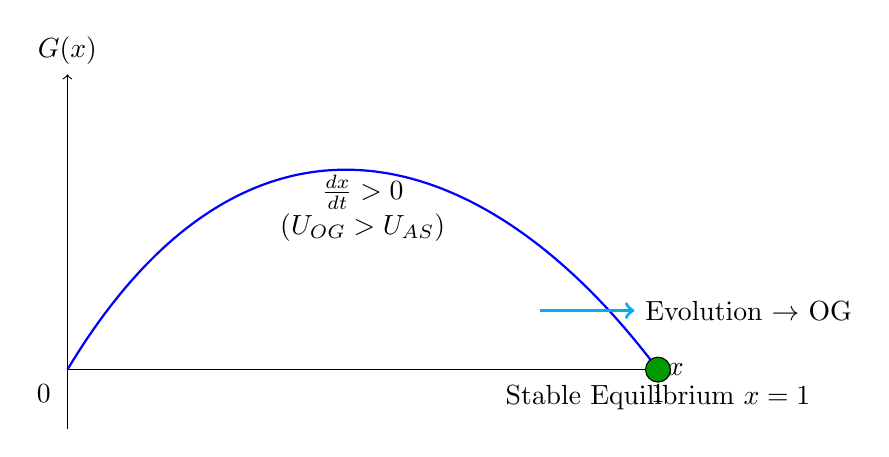
\begin{tikzpicture}[scale=1.5]
        % Axes
        \draw[->] (0,0) -- (5,0) node[right] {$x$};
        \draw[->] (0,-0.5) -- (0,2.5) node[above] {$G(x)$};
        \node at (5, -0.2) {1};
        \node at (-0.2, -0.2) {0};

        % Curve (Similar to Julian's plot, indicating OG dominance)
        \draw[thick, blue] (0,0) .. controls (1.5, 2.5) and (3.5, 2.0) .. (5,0.0);

        % Interpretation: Movement towards x=1
        \draw[->, cyan, very thick] (4, 0.5) -- (4.8, 0.5) node[right, black] {Evolution $\to$ OG};
        
        % Annotation: G(x) > 0 region
        \node at (2.5, 1.5) {$\frac{dx}{dt} > 0$};
        \node at (2.5, 1.2) {($U_{OG} > U_{AS}$)};
        
        % The point x=1 is the stable equilibrium
        \draw[fill=green!60!black] (5,0) circle (3pt);
        \node[below] at (5, -0.05) {Stable Equilibrium $x=1$};
    \end{tikzpicture}
    \caption{Visual representation of the Replicator Dynamics Speed $G(x)$. In this scenario (consistent with the results when $c \geq \lambda r$), $G(x)$ is non-negative, indicating that the OG strategy is evolutionarily superior, leading the population to converge towards the $x=1$ (Only Good) pure strategy equilibrium.}
    \label{fig:Gx_OG_Dominant}
\end{figure}

The standard form of the replicator equation for the frequency of strategy OG ($x$) is:

\begin{enumerate}
    \item \textbf{Standard Replicator Dynamics Equation}
    The fundamental principle states that the evolution speed of a strategy is proportional to its current proportion and its advantage relative to the average fitness of the population ($\bar{U}_A$).
    The standard replicator equation for the proportion $x$ of OG strategy is:
    $$\frac{dx}{dt} = x \cdot (U_{OG} - \bar{U}_A) \quad (\text{Equation } 1)$$
    where:
    \begin{itemize}
        \item $x$ is the proportion of OG strategy (i.e., $\theta_{OG}$).
        \item $U_{OG}$ is the fitness (Payoff) of the OG strategy.
        \item $\bar{U}_A$ is the average fitness of the author population.
    \end{itemize}
    
    \item \textbf{Average Population Payoff ($\bar{U}_A$) in the Two-Strategy Game}
    Since our model includes only two author strategies, OG (proportion $x$) and AS (proportion $1-x$), the average population fitness $\bar{U}_A$ is defined as the weighted average of the two payoffs:
    $$\bar{U}_A = x \cdot U_{OG} + (1-x) \cdot U_{AS}$$
    
    \item \textbf{Derivation of Equivalence}
    We substitute the expression for the average fitness $\bar{U}_A$ into the standard replicator equation (Equation 1):
    $$\frac{dx}{dt} = x \cdot \left[ U_{OG} - \left( x \cdot U_{OG} + (1-x) \cdot U_{AS} \right) \right]$$
    
    Next, we perform algebraic rearrangement:
    $$\frac{dx}{dt} = x \cdot \left( U_{OG} - x \cdot U_{OG} - (1-x) \cdot U_{AS} \right)$$
    
    We group the terms involving $U_{OG}$:
    $$\frac{dx}{dt} = x \cdot \left( U_{OG} \cdot (1-x) - U_{AS} \cdot (1-x) \right)$$
    
    Finally, factoring out the common term $(1-x)$ yields the simplified form of the replicator equation:
    $$\frac{dx}{dt} = x \cdot (1-x) \cdot (U_{OG} - U_{AS})$$
\end{enumerate}

The formula $G(x) = x(1-x) \cdot (U_{OG} - U_{AS})$ is thus mathematically equivalent to the standard replicator equation in this context. It is often preferred in two-strategy analysis because it directly relates the change in frequency ($\frac{dx}{dt}$) to the absolute payoff difference between the two competing strategies ($U_{OG} - U_{AS}$). The term $x(1-x)$ ensures the speed of evolution approaches zero near the pure strategy boundaries ($x=0$ or $x=1$).

\subsection{Visualizing the Evolutionary Dynamics $G(x)$ and the Role of Capacity $K$}

The attached Figure \ref{fig:Gx_K_Analysis} (GX\_and\_K.png) displays the evolutionary speed $G(x) = dx/dt$ as a function of the OG proportion ($x$) for varying journal capacities ($K$). The simulation used the following default parameters:
\begin{itemize}
    \item Population Size ($N$): $100$
    \item Good Paper Probability ($\alpha$): $0.6$
    \item Journal Strategy: Fixed at \textbf{Strict Selection} ($\phi_{OG} \approx 1$)
    \item Peer Review Noise ($\epsilon, \lambda$): $\epsilon = 0.1, \lambda = 0.1$
    \item Cost and Reward ($c, r$): $c=0.1, r=1.0$
\end{itemize}
\begin{figure}[h!]
    \centering
    \includegraphics[width=0.8\textwidth]{GX_and_K.png}
    \caption{Replicator Dynamics $G(x)$ for Varying Capacity $K$ (N=100, $\alpha=0.6$, Strict Journal)}
    \label{fig:Gx_K_Analysis}
\end{figure}



All curves in Figure \ref{fig:Gx_K_Analysis} remain non-negative, confirming that the \textbf{Only Good ($x=1$)} strategy is the globally stable evolutionary equilibrium (ESE) under these specific parameter settings, as $U_{OG} \ge U_{AS}$ across the entire strategy space.

The magnitude of $G(x)$ (the peak height of the curve) represents the \textbf{speed of convergence} towards the OG equilibrium.

\paragraph{Algebraic Role of Capacity $K$:}
The capacity $K$ is introduced via the expected competition factor $E[\gamma]$, which determines the true acceptance probability for any paper that passes peer review. The difference in fitness between the two strategies is proportional to the term $\left( c - \lambda r E[\gamma] \right)$.

The competition factor $E[\gamma]$ is defined as:
$$E[\gamma] = E\left[\min\left(1, \frac{\mathbf{K}}{1+M_{-i}}\right)\right]$$

\paragraph{Resulting Curve Changes:}
\begin{enumerate}
    \item \textbf{High $K$ (e.g., $K=70$):} When $K$ is large, the competition factor $E[\gamma]$ is close to $1$ for most $x$ values (Resource Abundance regime). With $c=\lambda r=0.1$ in this scenario, the payoff difference is minimized ($\Delta U \approx 0$). This results in the \textbf{flattest curve} with the lowest convergence speed.
    \item \textbf{Low $K$ (e.g., $K=10$):} When $K$ is small, the system is highly congested (Resource Scarcity regime). Since $E[\gamma]$ is small, the payoff difference $\Delta U > 0$ is maximized. This leads to the \textbf{steepest curve} and the fastest evolutionary speed toward OG. The scarcity of slots ($K$) enhances the relative advantage of the higher-quality strategy (OG), promoting quick convergence to cooperation.
\end{enumerate}


The analysis of the Threshold Competition Model focuses on how the intrinsic quality of authors, represented by the probability of producing a good paper ($\alpha$), shapes the speed of evolutionary convergence.



The analysis of the Threshold Competition Model focuses on how the intrinsic quality of authors, represented by the probability of producing a good paper ($\alpha$), shapes the speed of evolutionary convergence.

\subsection{Visualization of $G(x)$ for Varying $\alpha$}

Figure \ref{fig:Gx_alpha_Analysis} displays the evolutionary speed $G(x)$ across the entire spectrum of author strategy mixes ($x = \theta_{OG}$) for different values of $\alpha$.

\begin{figure}[h!]
    \centering
    \includegraphics[width=0.8\textwidth]{GX_alpha.png}
    \caption{Author Replicator Dynamics $G(x)$ for Varying Good Paper Rate $\alpha$ (Fixed $N=100, K=20, c=0.1, \lambda=0.1$)}
    \label{fig:Gx_alpha_Analysis}
\end{figure}



The simulation holds several parameters fixed to isolate the effect of $\alpha$:
\begin{itemize}
    \item Fixed Capacity ($K$): $20$
    \item Fixed Cost and Noise: $c=0.1$, $\epsilon=0.1$, and $\lambda=0.1$.
    \item Fixed Journal Strategy: $\phi_{OG} \approx 0.999$ (Strict Selection).
\end{itemize}

Since all curves remain non-negative ($G(x) \ge 0$) across the entire range $x \in (0, 1)$, the only stable equilibrium is the \textbf{Pure Only Good (OG) equilibrium} at $x=1$. This confirms that under these costs ($c=\lambda r=0.1$), the OG strategy is evolutionarily superior, and the population will converge to full cooperation.



The magnitude of the evolutionary speed $G(x)$ is directly proportional to the payoff difference $\Delta U = U_{OG} - U_{AS}$. This difference, derived from the core expected payoff functions, is governed by $\alpha$ through two competing mechanisms:


The payoff difference $\Delta U$ simplifies to:
$$\Delta U \propto \mathbf{(1-\alpha)} \cdot \left( c - \lambda \cdot E[\gamma] \cdot r \right)$$

\begin{enumerate}
    \item \textbf{Scaling Factor ($\mathbf{1-\alpha}$):} This term dictates the overall magnitude of the difference. As $\alpha$ increases towards $1$, this scaling factor approaches zero, mechanically \textbf{reducing} the amplitude of $G(x)$. This explains the final decline of the curve magnitude when $\alpha$ is very high (e.g., $\alpha=0.9$).
    
    \item \textbf{Absolute Payoff of OG ($\mathbf{\alpha}$):} $\alpha$ is also the probability that an OG author submits and potentially receives the reward. Increasing $\alpha$ (from $0.01$ to $0.5$) significantly boosts the absolute value of $U_{OG}$, while the costs are fixed. This drives the initial \textbf{increase} in $\Delta U$ and thus the peak height of $G(x)$.
\end{enumerate}

The non-monotonic shape (rising steeply and then falling) is a result of the competition between the initial benefit boost from a higher $\alpha$ and the subsequent dampening effect from the reduced scaling factor $(1-\alpha)$.


The fastest transition to a cooperative equilibrium occurs when authors are intrinsically capable ($\alpha$ is high), but the remaining small chance of submitting a bad paper still provides a sufficiently strong selective pressure against the indiscriminate Always Submit strategy.

\subsection{Conclusion on Evolutionary Stability and Theoretical Constraints}

The collective results from simulating the effects of capacity $K$ and intrinsic quality $\alpha$ on the evolutionary speed $G(x)$ yield a consistent finding: $\mathbf{G(x) \ge 0}$ across all simulated parameter combinations ($x \in [0, 1]$).



The observation that $G(x)$ is always non-negative implies:
\begin{enumerate}
    \item \textbf{Evolutionary Dominance:} The payoff of the Only Good (OG) strategy is always greater than or equal to the payoff of the Always Submit (AS) strategy ($U_{OG} \ge U_{AS}$).
    \item \textbf{Convergence:} The population will inevitably evolve towards the \textbf{Pure Only Good (OG) equilibrium} ($x=1$).
\end{enumerate}


If $G(x)$ were negative in any region, it would mean that the Always Submit strategy provides a higher payoff than the Only Good strategy ($U_{AS} > U_{OG}$), driving the population towards the pure AS equilibrium ($x=0$).



The consistent result of $G(x) \ge 0$ is a direct consequence of the parameters chosen in the simulation, which were selected to respect the simplified $2 \times 2$ game structure. The critical condition is derived from comparing the submission cost ($c$) to the potential reward from a lucky acceptance:
$$U_{OG} - U_{AS} \propto \left( c - \lambda \cdot E[\gamma] \cdot r \right)$$

For $G(x)$ to be negative, the AS strategy must be dominant, requiring $\mathbf{c < \lambda \cdot E[\gamma] \cdot r}$. Since the maximum value of the competition factor $E[\gamma]$ is $1.0$, this can only occur if $\mathbf{c < \lambda r}$.

The simulation parameters adhere to the boundary case of the \textbf{Constraint 1} defined earlier:
\begin{itemize}
    \item \textbf{Constraint 1:} $\mathbf{c > \lambda r}$ (Designed to prevent the malicious OB strategy from being rational).
    \item \textbf{Simulated Value:} The fixed parameters $c=0.1$ and $\lambda r = 0.1 \cdot 1.0 = 0.1$ result in $\mathbf{c = \lambda r}$.
\end{itemize}

The condition $\mathbf{c = \lambda r}$ is a critical boundary condition where the expected payoff of submitting a bad paper (through $\lambda$) exactly equals the submission cost. This forces the term $(c - \lambda \cdot E[\gamma] \cdot r)$ to be non-negative, as $E[\gamma] \le 1$.

In essence, the initial theoretical condition designed to guarantee the validity of the simplified $2 \times 2$ game (by eliminating OB) also \textbf{constrains the evolutionary dynamics to only favor the OG strategy}, thus preventing $G(x)$ from becoming negative.



\section{Evolutionary Dynamics Analysis under Capacity Constraint}


The simulation utilizes the Threshold Competition Model with $N=100$ authors, a fixed capacity $K=20$, a high reward $r=1.0$, moderate cost $c=0.1$, a baseline good paper rate $\alpha=0.6$, and peer review noise set at $\epsilon=\lambda=0.1$, coupled with a strong journal penalty $D=3.0$ for accepting bad papers.


The provided time-series plot confirms the system's strong overall drive towards cooperation. The proportion of Only Good (OG) authors ($\theta_{OG}$) quickly rises toward $0.9$, while the Always Submit (AS) share ($\theta_{AS}$) drops quickly towards $0.1$.

\begin{figure}[h]
    \centering
    \includegraphics[width=0.8\textwidth]{replicator dynamics.png}
    \caption{Author Replicator Dynamics (Multiple Runs, $\alpha=0.6$)}
    \label{fig:replicator_dynamics}
\end{figure}


Contrary to the initial expectation, after the rapid ascent, the $\theta_{OG}$ share does not monotonically increase to the boundary $1.0$, but instead enters a **prolonged floating or oscillatory state** between approximately $0.85$ and $0.95$.


This floating state appears inconsistent with previous static analyses which, under strict journal selection ($\phi_{OG} \approx 1$), showed that the author replicator dynamic $G(x) = dx/dt$ remains strictly positive ($G(x) > 0$) across the relevant range of $x=\theta_{OG}$, implying continuous convergence towards the cooperative boundary $x=1$ without oscillation.



The discrepancy strongly suggests a limitation in the standard static replicator analysis when applied to this specific co-evolutionary game. The floating behavior must arise from the **coupling** between the fast-evolving Journal strategy ($\phi_{OG}$) and the slow-evolving Author strategy ($\theta_{AS}$).

The primary suspect for driving this oscillation is the non-linear dependency of the Author payoff on the **Expected Competition Factor ($E[\gamma]$):**

The author's evolutionary speed is driven by the payoff difference:
$$
\frac{d\theta_{OG}}{dt} \propto (u_{OG} - u_{AS})
$$

\begin{enumerate}
    \item \textbf{High $\theta_{OG}$ Temporarily Lowers Congestion:} When $\theta_{OG}$ becomes very high (e.g., $\approx 0.9$), the population is mostly cooperative, resulting in fewer submissions that pass review. This temporarily \textbf{reduces system congestion} and pushes the Expected Competition Factor $E[\gamma]$ towards $1$.
    \item \textbf{AS Exploits High $E[\gamma]$:} This window of low congestion briefly makes the Always Submit ($AS$) strategy profitable, as its submission success probability $P_{pass}(AS)$ is inherently higher due to exploiting the false positive rate $\lambda$.
    \item \textbf{Payoff Reversal:} This temporary advantage causes $u_{AS}$ to briefly exceed $u_{OG}$, making the derivative $d\theta_{OG}/dt$ momentarily \textbf{negative}. The OG share retreats slightly, congestion immediately increases, and the $u_{OG} - u_{AS}$ term reverts to positive, driving $\theta_{OG}$ back up. This continuous cycle results in the observed floating around a quasi-equilibrium state near $x \approx 0.9$.
\end{enumerate}

This complex feedback loop confirms that the system's "Tragedy of the Commons" element is always active, leading to a dynamic rather than absolute stability at the cooperative boundary.

\end{document}



